\section{Implementierung}
In diesem Kapitel wird die Implementierung der hochselektiven Filterbank in Python 3.7 beschrieben.

\subsection{Übersicht}\label{sec:impl_ueber}

\subsubsection{Verwendete Bibliotheken}\label{sec:impl_bib}
Für einige Berechnungen und das Speichern von Datenstruckturen wurde das Numpy Modul der Scipy Bibliothek~\cite{scipy} verwendet. Für das Erstellen der Diagramme wurde die Matplotlib Bibliothek~\cite{Hunter:2007}.
\subsubsection{Klassendiagramm}\label{sec:impl_klass}
\begin{figure}
  \centering
  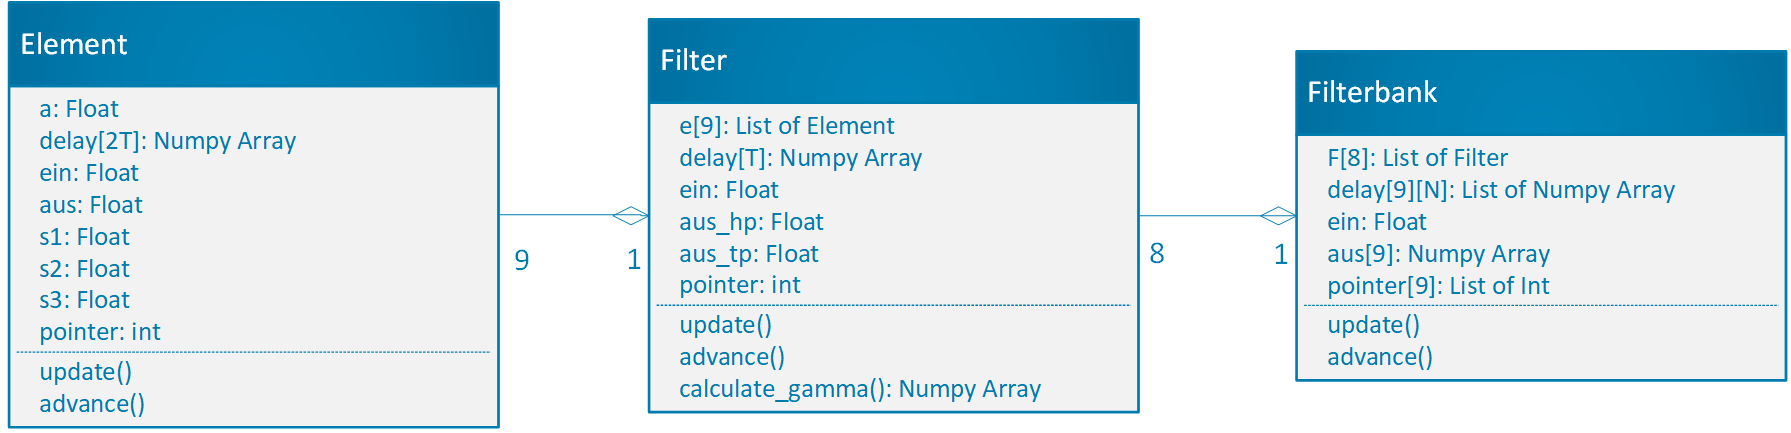
\includegraphics[width=1\textwidth]{img/klassendia}
  \caption{Klassendiagramm für die Implementierung einer hochselektiven Filterbank}\label{fig:impl_klassdia}
\end{figure}
Wie in Abbildung~\ref{fig:impl_klassdia} zu sehen erfolgt die Implementierung der hochselektiven Filterbank objektorientiert. Dabei besteht eine Filterbank aus 8 Filtern (vgl. Abb. TODO) und ein Filter aus 9 Elementen (vgl. Abb.).
\subsection{Klassen}\label{sec:impl_klassen}
Im folgenden wird die Implementierung der Klassen im einzelnen beschrieben bevor im nächsten Unterkaptitel auf dei verwendeten Testfunktionen eingegangen wird.
\subsubsection{Element}\label{sec:impl_ele}
Ein Element stellt den kleinsten Teil der Filterbank dar. Neben Ein- und Ausgang verfügt ein Element über ein Delay-Array dessen Länge eingestellt werden kann. Hierüber lässt sich die Ordnung des Teilfilters einstellen (vlg. Kap. TODO).

\lstinputlisting[language=Python, firstline=6, lastline=31, caption={Quellcode der Klasse Element}, label={lst:element}]{list/wellendigitalfilter.py}


\subsubsection{Filter}\label{sec:impl_Filter}
\lstinputlisting[language=Python, firstline=34, lastline=118, caption={Quellcode der Klasse Filter}, label={lst:filter}]{list/wellendigitalfilter.py}

\subsubsection{Filterbank}\label{sec:impl_bank}
\lstinputlisting[language=Python, firstline=121, lastline=160, caption={Quellcode der Klasse Filterbank}, label={lst:bank}]{list/wellendigitalfilter.py}
\subsection{Testfunktionen}\label{sec:impl_test}

\subsubsection{Test Filter}\label{sec:impl_testFilter}
\lstinputlisting[language=Python, firstline=163, lastline=193, caption={Quellcode der Testfunktion für einen einzlnen Filter}, label={lst:test_filter}]{list/wellendigitalfilter.py}
\subsubsection{Test Filterbank}\label{sec:impl_testBank}
\lstinputlisting[language=Python, firstline=196, lastline=236, caption={Quellcode der Testfunktion für die gesamte Filterbank}, label={lst:element}]{list/wellendigitalfilter.py}
%%% Local Variables:
%%% mode: latex
%%% TeX-master: "../termpaper"
%%% End:
